% LaTeX Article Template
\documentclass[12pt]{article}
%% Other packages
\usepackage{amsmath}
\usepackage{amsthm}
\usepackage{titlesec}
\usepackage{soul}
\usepackage{tikz}
\usepackage{tikz-3dplot}
\usepackage{amssymb}
\usepackage{multicol}
\usepackage{algorithm}
\usepackage{algorithmic}
\usepackage{float}
\usepackage{calc}
\usepackage{fancybox}
\usepackage{array}
\usepackage[shortlabels]{enumitem}
\usepackage{framed}
\usepackage{hyperref}
\newcolumntype{L}[1]{>{\raggedright\let\newline\\\arraybackslash\hspace{0pt}}m{#1}}
\newcolumntype{C}[1]{>{\centering\let\newline\\\arraybackslash\hspace{0pt}}m{#1}}
\newcolumntype{R}[1]{>{\raggedleft\let\newline\\\arraybackslash\hspace{0pt}}m{#1}}


%% Margins
\usepackage{geometry}
\geometry{verbose,letterpaper,tmargin=1in,bmargin=1in,lmargin=1in,rmargin=1in}

\newcommand{\menuchoice}[2]{{\ttfamily#1..#2}}
\newcommand{\dotdot}{..}

\usepackage{graphicx}

% Array vertical and horizontal stretch
% \def\arraystretch{1.5}%  1 is the default, change whatever you need
% \setlength{\tabcolsep}{12pt}

%\graphicspath{%
\graphicspath{{./figs/}}

%% Paragraph style settings
\setlength{\parskip}{\medskipamount}
\setlength{\parindent}{0pt}

%% Change itemize bullets
\renewcommand{\labelitemi}{$\bullet$}
\renewcommand{\labelitemii}{$\circ$}
\renewcommand{\labelitemiii}{$\diamond$}
\renewcommand{\labelitemiv}{$\cdot$}

%% Shrink section fonts
\titleformat*{\section}{\large\bf}
\titleformat*{\subsection}{\normalsize\it}
\titleformat*{\subsubsection}{\normalsize\bf}

% %% Compress the spacing around section titles
\titlespacing*{\section}{0pt}{1.5ex}{0.75ex}
\titlespacing*{\subsection}{0pt}{1ex}{0.5ex}
\titlespacing*{\subsubsection}{0pt}{1ex}{0.5ex}

%% amsthm settings
\theoremstyle{definition}
\newtheorem{problem}{Problem}
\newtheorem{example}{Example}
\newtheorem{mydef}{Definition}

%% Answer box macros
%% \answerbox{alignment}{width}{height}
\newcommand{\answerbox}[3]{%
  \fbox{%
    \begin{minipage}[#1]{#2}
      \hfill\vspace{#3}
    \end{minipage}
  }
}

%% \answerboxfull{alignment}{height}
\newcommand{\answerboxfull}[2]{%
  \answerbox{#1}{\textwidth}{#2} 
}

%% \answerboxone{alignment}{height} -- for first-level bullet
\newcommand{\answerboxone}[2]{%
  \answerbox{#1}{6.15in}{#2} 
}

%% \answerboxtwo{alignment}{height} -- for second-level bullet
\newcommand{\answerboxtwo}[2]{%
  \answerbox{#1}{5.8in}{#2}
}

%% \graphbox{xmin}{xmax}{ymin}{ymax}{scale}
\newcommand{\graphbox}[5]%[-5, 5, -5, 5, 0.33]
{
\begin{tikzpicture}
     [>=latex,scale=#5]
     
     % Coordinate axes
     \draw [->,very thick] (#1, 0) -- (#2, 0) node[right] {$x$};
     \draw [->,very thick] (0, #3) -- (0, #4) node[above] {$y$};
     
     % Grid
     \draw[step=1cm,thick,dotted] (#1,#3) grid (#2,#4);
   \end{tikzpicture}
   }


%% Redefine maketitle
\makeatletter
\renewcommand{\maketitle}{
  \noindent SA403 -- Networks \\

  \begin{center}\Large{\textbf{\@title}}\end{center}
}
\makeatother

% Set the beginning of a LaTeX document
\begin{document}

%\graphbox{-10}{3}{-5}{10}

\title{Lesson: Depth and Breadth First Search Algorithms}

%\graphbox[10][10]

\maketitle


%\section*{Notes}

%Book acknowledgment: 
\section*{Goals}
\begin{itemize}
\item Breadth First Search
\item Depth First Search
\end{itemize}

\section{COVID-19 Contact Tracing Example}

Suppose that there is an outbreak of COVID-19 within a small group of the $1^{st}$ company. We want to conduct a contact tracing study to see who needs to quarantine. Consider the following details.

\begin{itemize}
	\item We know that Professor Curry contracted COVID-19. (I don't have COVID-19. This is just an example.)
	\item We want to study a small group of ten possible mids that \emph{could} because they are supposed to be traveling on an MO tomorrow. If they are found in the contact tracing tree, then they are unable to go on the MO. Set of students $\{$Jim, Dre, Sean, Connor, Ana, Caroline, Mike, Jayla, Xavier, Ashley$\}$. 
	\item We know that Jayla, Xavier, and Caroline were all in Prof Curry's office without masks on.
	\item Jayla, Caroline, and Ana are all roommates.
	\item Xavier and Mike are roommates.
	\item Mike, Xavier, and Connor all ate lunch inside together today.
\end{itemize}
\newpage

\begin{enumerate}
	\item Given what you know now about algorithms, formulate an algorithm for solving this problem. 
\end{enumerate}

\section{Family Tree Example}

Let's take a look at another example. We want to come up with an algorithm for creating a visual representation of the Simpson's family tree. Here's the relevant information:
\begin{itemize}
	\item Abraham and Mona are Herb and Homer's parents.
	\item Clancy and Jackie are Marge, Patty, and Selma's parents.
	\item Homer and Marge are Bart, Lisa, and Maggie's parents.
	\item Selma is Ling's Parent.
\end{itemize} 

\begin{enumerate}
	\item Create a visual representation of the Simpson's family tree.
	\vfill
	\item Number each family member in the order in which you drew them.
	\vfill
\end{enumerate}

\newpage
\section{Now, let's work backwards...}

Consider the visual representation of (a portion of) the Potter and Malfoy family tree. (Image credit from Reddit)

\begin{center}
\includegraphics[width=8cm]{potter_family_tree}
\end{center}

\begin{enumerate}
	
\item Systemically determine the parent of each character depicted in the tree above.
\end{enumerate}
\vfill
\newpage

%\section{Try it on your own}

%Given some graph $G = (V,E)$, how would you systematically explore and number all the connected nodes in $V$?

%Try it on this example:

%\begin{center}
%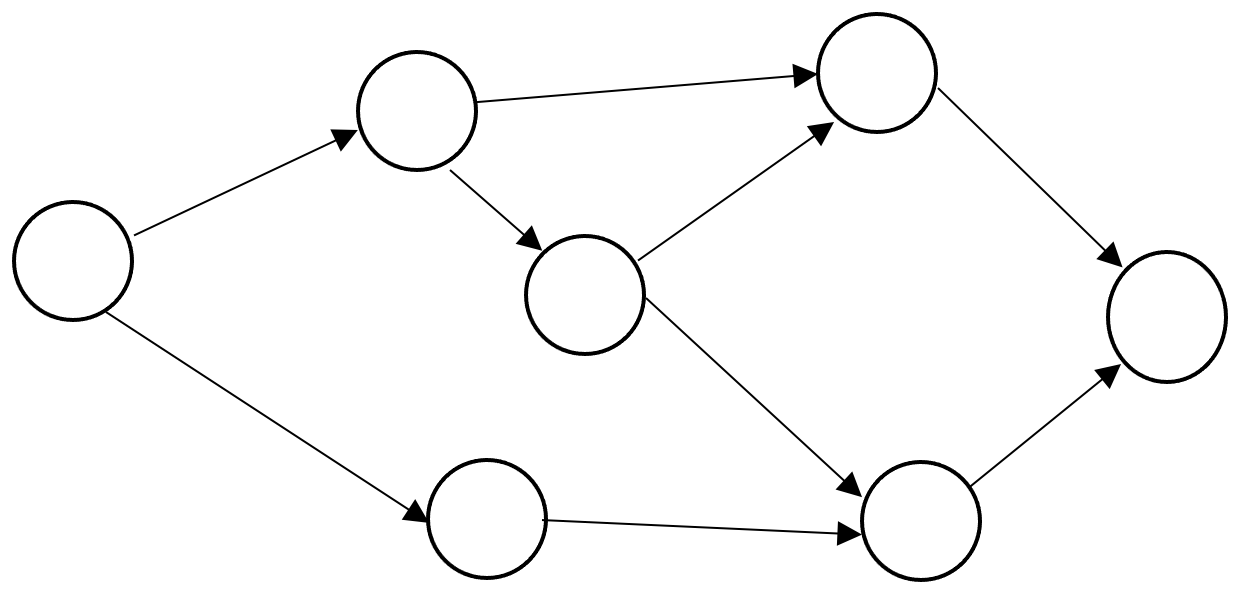
\includegraphics[width=10cm]{searchgraph}
%\end{center}

%Write down your steps below:
%\newpage


\section{Search Algorithms}

Given $s$ as the source node, the two search algorithms we study in this lession will systematically explore the edges of $G$ to \emph{discover} every node that is reachable from $s$. They also calculate the fewest number of edges from $s$ to each reachable node in $G$. While very similar, these two search algorithms differ in implementation and analysis.

\subsection{Breadth First Search}

You can think of the Bread First Search (BFS) algorithm that explores each \emph{layer} of the network.

To simplify this algorithm, the BFS signifies each node as \emph{explored} when found in the tree. 

\begin{itemize}
\item All nodes start as unexplored and may later be explored. 
\item The BFS will keep up with a queue $Q$ that keeps up with the list of nodes that should be explored next.
\end{itemize}


The BFS constructs a BF \emph{\textbf{tree}}, initially containing only its root node $s$. Whenever the search encounters an unexplored node $v$ in the course of scanning the adjacency list of an already encountered node $u$, the node $v$ and the edge $(u,v)$ are added to the tree. Thus, we refer to the node $u$ as the \textbf{\emph{parent}} of $v$. Since a node is discovered at most once, then each node has at most one parent. 

\vfill
What do you think are the pros and cons of the BFS algorithm?

\vfill
Questions?

\vfill
\newpage

\emph{\textbf{Written Steps:}}

\vskip .25cm

Initialization: Create queue $Q = \emptyset$. Add source node $s$ to $Q$, and mark $s$ as explored.
\begin{enumerate}
	\item If $Q$ is empty, then proceed to Step \ref{Step3}. Otherwise, remove node $v$ from the bottom of $Q$. Proceed to Step \ref{Step2}. \label{Step1}
	\item For some adjacent node $w \in V$ of $v$, if $w$ is not explored, then add $w$ to the bottom/end of $Q$, mark $w$ as explored, and set the parent of $w$ to be $v$. Repeat Step \ref{Step2}. \label{Step2}
	\item Terminate the algorithm with the BF tree resulting from the parent vector of each node in $V$. \label{Step3}
\end{enumerate}

\emph{\textbf{Pseudocode:}}


\begin{algorithm}[h]
\caption{Determine a BF tree for the Graph $G$ with source node $s$}
\begin{algorithmic} 
%\REQUIRE $n \geq 0 \vee x \neq 0$
%\ENSURE $y = x^n$
\STATE Let $Q$ be the queue
\STATE Add $s$ to $Q$.
\STATE Mark $s$ as explored.
\WHILE{$Q$ is not empty}
	\STATE Remove $v$ from $Q$
	\FOR{all adjacent nodes $w \in \mathcal{V}$ of $v$ }
		\IF{$w$ is not explored}
			\STATE Add $w$ to $Q$
			\STATE Mark $w$ as explored
			\STATE Mark $v$ as the parent of $w$
		\ENDIF
	\ENDFOR

\ENDWHILE
\end{algorithmic}
\end{algorithm}



Run the BFS algorithm on the following graph:

\begin{center}
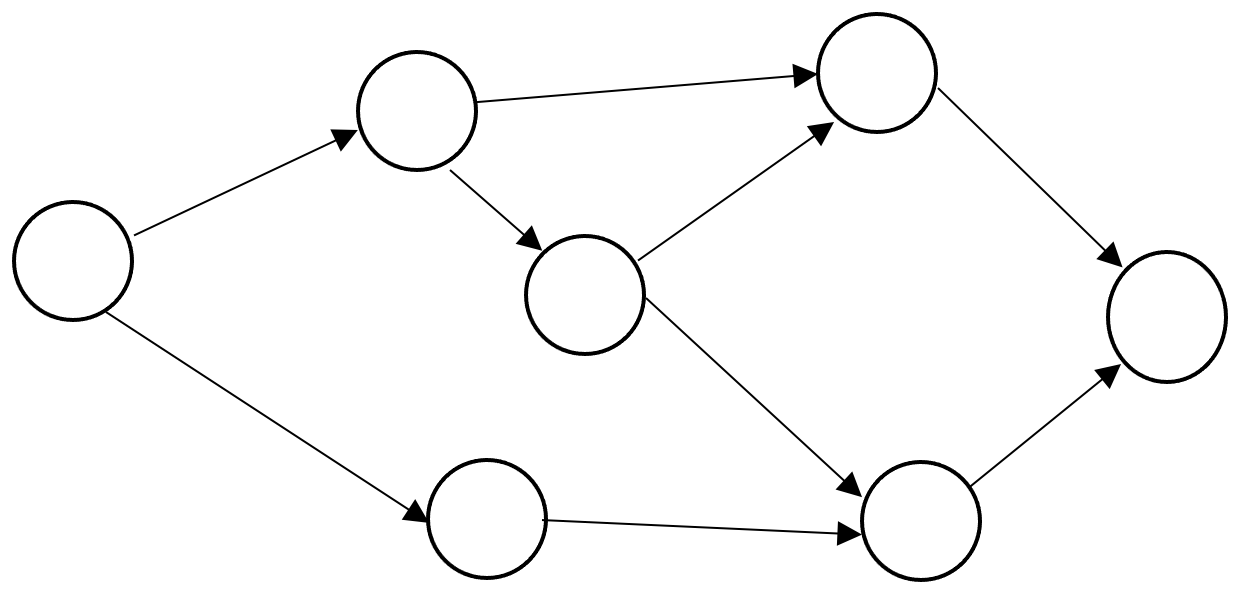
\includegraphics[width=10cm]{searchgraph}
\end{center}

\newpage

\section{Depth First Search}

Given the name of the Depth First Search (DFS), how do you think it differs from the BFS?

Just like the BFS algorithm, the DFS algorithm also constructs a \emph{\textbf{tree}}, initially containing only its root node $s$. Rather than exploring the \emph{layers} of the graph (as with the BFS algorithm) by exploring \textbf{all} adjacent nodes of each node before moving to another node, the DFS instead continually explores a series of adjacent nodes until the algorithm reaches a node having no adjancent nodes (also known as a leaf node). The DFS algorithm is a repetitive algorithm that \emph{backtracks} to a recently visited node. 
\vfill

What do you think are the pros and cons of the BFS algorithm?

\vfill
Questions?

\vfill

\emph{\textbf{Written Steps:}}

\vskip .25cm

Initialization: Create stack $S = \emptyset$. Add source node $s$ to the top of $S$, and mark $s$ as explored.
\begin{enumerate}
	\item If $S$ is empty, then proceed to Step \ref{Step3}. Otherwise, remove node $v$ from the top of $S$. Proceed to Step \ref{Step2}. \label{Step1}
	\item For each adjacent node $w \in V$ of $v$,  add $w$ to the top of $S$ and set the parent of $w$ to be $v$. Otherwise, repeat Step \ref{Step2}. \label{Step2}
	\item Terminate the algorithm with the DF tree resulting from the parent vector of each node in $V$. \label{Step3}
\end{enumerate}


\emph{\textbf{Pseudocode:}}


\begin{algorithm}
\caption{Determine a DF tree for the Graph $G$ with source node $s$}
\begin{algorithmic} 
\STATE Let $S$ be a stack.
\STATE Insert $s$ at the top of $S$.
\WHILE{$S$ is not empty}
	\STATE Remove node $v$ from the top of $S$
	\FOR{all adjacent nodes $w \in \mathcal{V}$ of $v$ }
		\STATE Add $w$ to the top $S$
		\STATE Mark $v$ as the parent of $w$
	\ENDFOR

\ENDWHILE
\end{algorithmic}
\end{algorithm}

\newpage

Run the DFS algorithm on the following graph:

\begin{center}
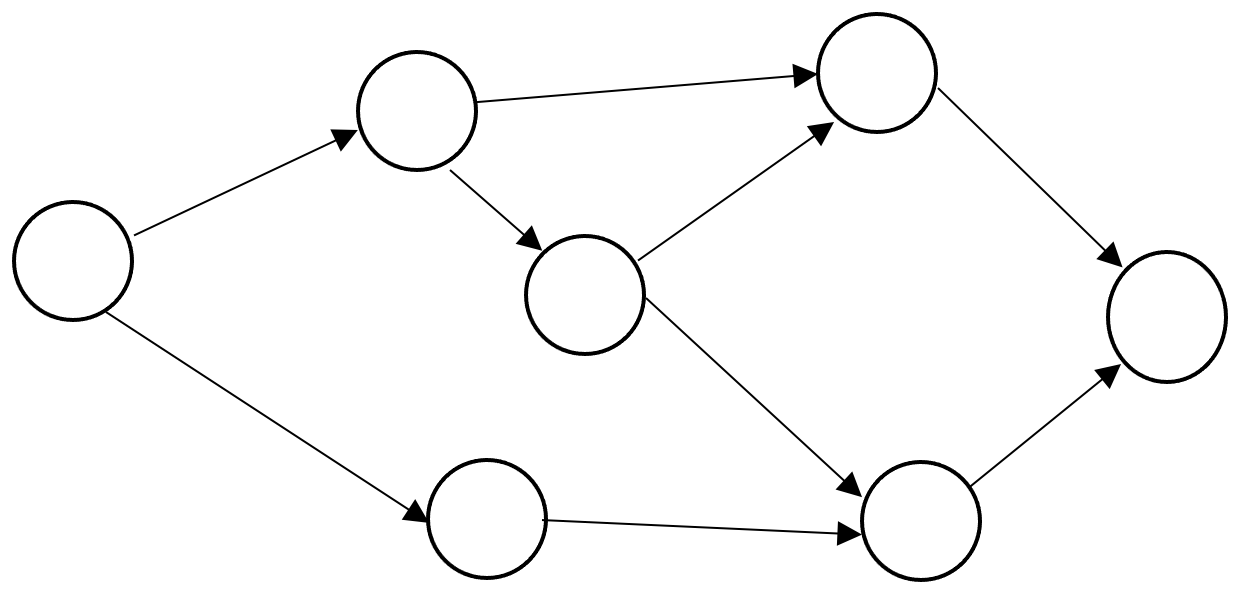
\includegraphics[width=10cm]{searchgraph}
\end{center}



\end{document}
